\documentclass[]{article}
\usepackage{graphicx}
\graphicspath{{../CMS_Plots/}, {../CMS_Events/}}
%opening
\title{Jerrod Thesis Outline}
\author{Jerrod T. Dixon}

\begin{document}

\maketitle

\section{Introduction}

\section{Background}
\subsection{WLCG Network Grid}
\subsubsection{Involved Facilities}
\subsubsection{CMS Experiment}
\subsection{Nature of WLCG jobs}
\subsubsection{Condor}
Purpose, HTC model, etc.
\subsubsection{Important properties}
Mention the different fields (CpuEff, EventRate) interested in
\subsection{Importance of reported values}
\subsection{Motivation}
\section{Related Work}
\subsection{Atlas MWT2}
\subsubsection{Elasticsearch}
\subsubsection{PerfSONAR}
\subsection{CERN CMS experiment}
\section{Experiment on CMS performance}
\subsection{Setup}
\subsubsection{Aggregation of Condor databases}
\subsubsection{Elasticsearch servers}
\subsection{Processing method of data}
\section{Results}
\subsection{Effects on job performance}
\subsection{Packet Loss}
\subsubsection{Effect on CpuEff}
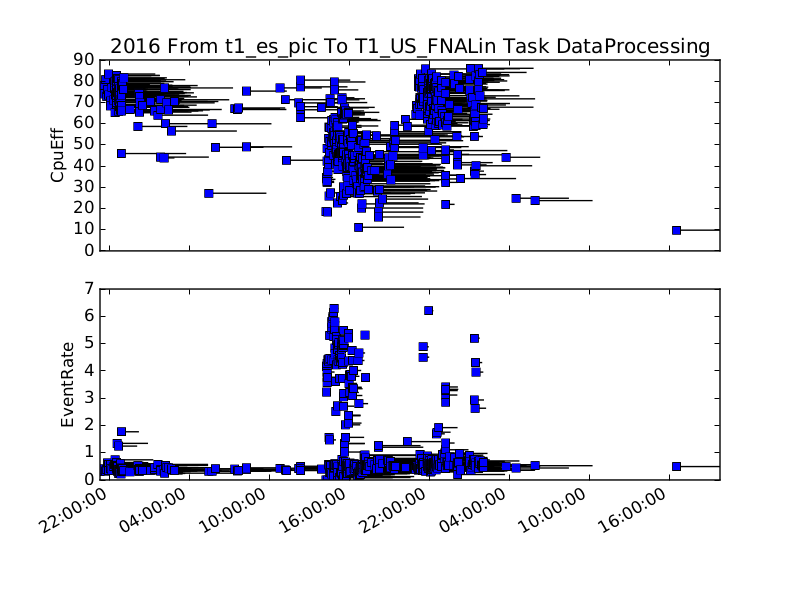
\includegraphics[scale=0.5]{CpuEff_EventRate_pic_FNAL}
\subsubsection{Effect on EventRate}
\subsection{Latency}
\subsubsection{Effect on CpuEff}
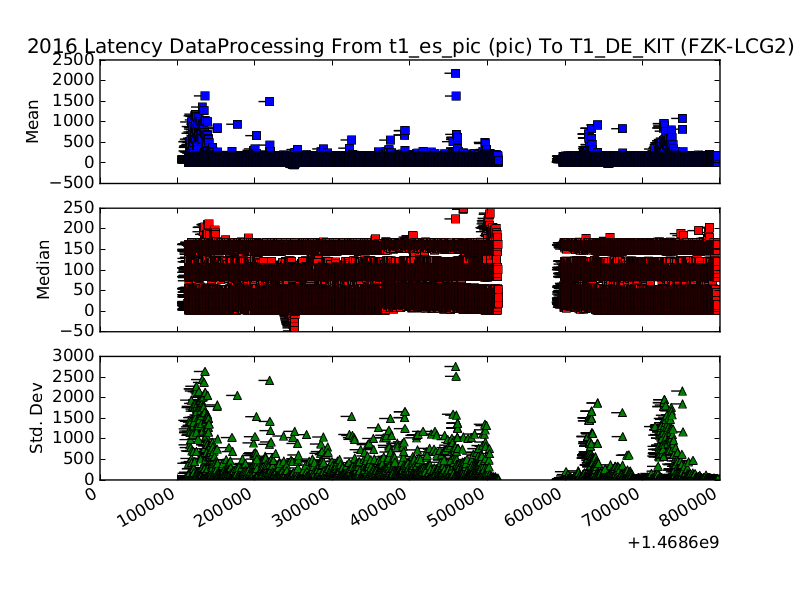
\includegraphics[scale=0.5]{Latency_pic_kit}
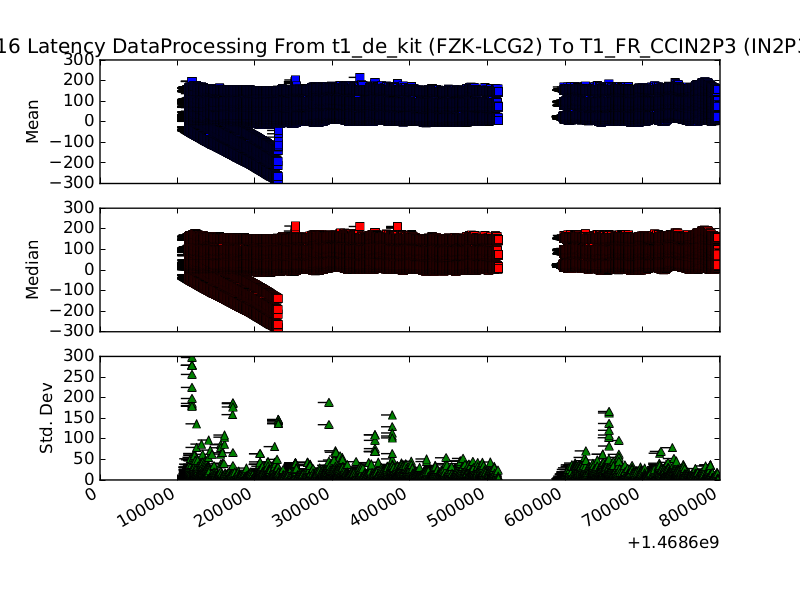
\includegraphics[scale=0.5]{Latency_kit_CCIN2P3}
\subsubsection{Effect on EventRate}
\subsection{Throughput}
\subsubsection{Effect on CpuEff}
\subsubsection{Effect on EventRate}
\section{Conclusions and Future Work}
\subsection{Side discoveries}
\subsubsection{Drop in EventRate against CpuEff}
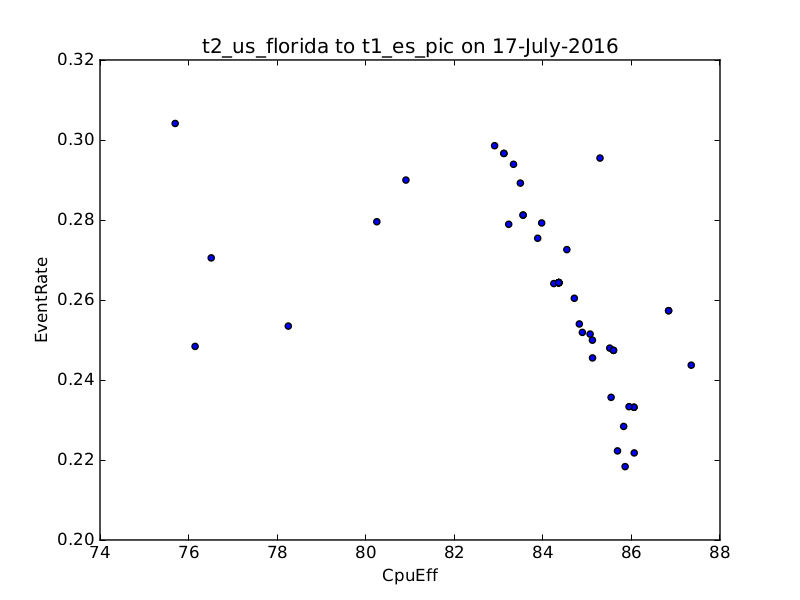
\includegraphics[scale=0.5]{CpuEff_EventRate_florida_pic_17July}
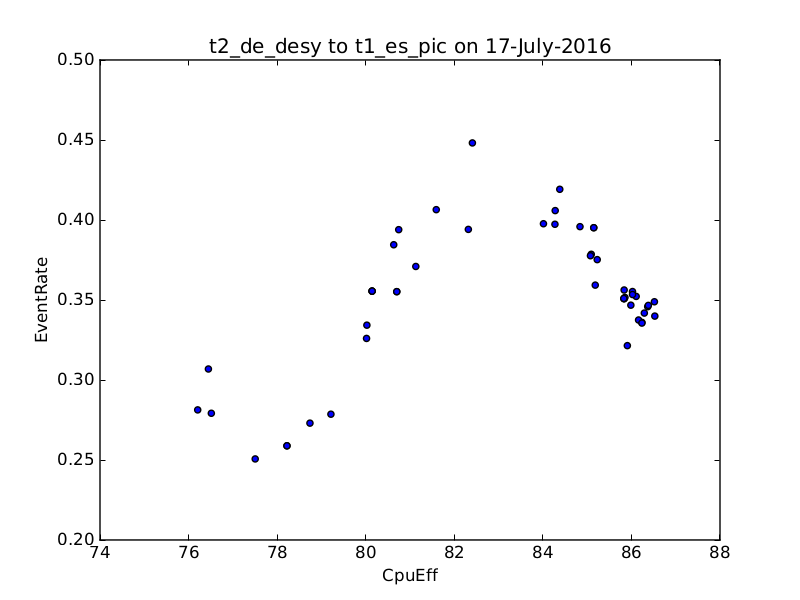
\includegraphics[scale=0.5]{CpuEff_EventRate_desy_pic_17july}
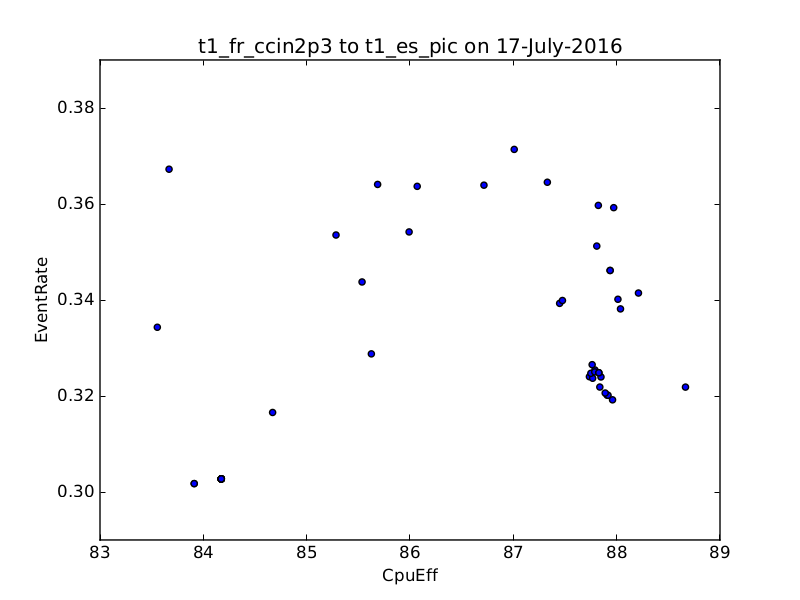
\includegraphics[scale=0.5]{CpuEff_EventRate_ccin2p3_pic_17july}
\end{document}
